% questions.tex —— 2002 年·苏豫粤桂卷 · 题目内容片段（无答案）
% 由 tools/generate_projects.py 依来源总账自 2002/2002_数学真题_苏豫粤桂_试题.md 生成，勿手改（改源 MD 后重跑）


\begin{gktip}
来源说明：本稿只转录固定 PDF 中可见的 Q1–Q22；原件为两页 A3 横向，印刷页 113–114。题签未标文理轨道，本文不推断适用范围；来源发布者、出版者、版次、复制链和官方身份仍未核。固定 PDF 没有答案或评分页，官方答案未认证。Q10、Q19、Q21 原页图已按固定文件矢量重绘；Q21 解析中的剪线图为本库作答辅助，不是原卷所印图。
\end{gktip}

\gkpart{一、选择题}

\begin{question}
\gkti{1}函数
\nopagebreak[4]
\[
f(x)=\frac{\sin 2x}{\cos x}
\]
的最小正周期是\mbox{（　　）}

(A) $\dfrac{\pi}{2}$　　(B) $\pi$　　(C) $2\pi$　　(D) $4\pi$

\end{question}
\begin{question}
\gkti{2}圆 $(x-1)^2+y^2=1$ 的圆心到直线 $y=\dfrac{\sqrt3}{3}x$ 的距离是\mbox{（　　）}

(A) $\dfrac12$　　(B) $\dfrac{\sqrt3}{2}$　　(C) $1$　　(D) $\sqrt3$

\end{question}
\begin{question}
\gkti{3}不等式 $(1+x)(1-|x|)>0$ 的解集是\mbox{（　　）}

(A) $\{x\mid 0\leqslant x<1\}$　　(B) $\{x\mid x<0\text{ \text{且} }x\ne-1\}$

(C) $\{x\mid -1<x<1\}$　　(D) $\{x\mid x<1\text{ \text{且} }x\ne-1\}$

\end{question}
\begin{question}
\gkti{4}在 $(0,2\pi)$ 内，使 $\sin x>\cos x$ 成立的 $x$ 的取值范围是\mbox{（　　）}

(A) $\left(\dfrac\pi4,\dfrac\pi2\right)\cup\left(\pi,\dfrac{5\pi}4\right)$

(B) $\left(\dfrac\pi4,\pi\right)$

(C) $\left(\dfrac\pi4,\dfrac{5\pi}4\right)$

(D) $\left(\dfrac\pi4,\pi\right)\cup\left(\dfrac{5\pi}4,\dfrac{3\pi}2\right)$

\end{question}
\begin{question}
\gkti{5}设集合
\nopagebreak[4]
\[
M=\left\{x\middle|x=\frac{k}{2}+\frac14,\ k\in\mathbb Z\right\},\qquad
N=\left\{x\middle|x=\frac{k}{4}+\frac12,\ k\in\mathbb Z\right\},
\]
则\mbox{（　　）}

(A) $M=N$　　(B) $M\subseteq N$　　(C) $M\supseteq N$　　(D) $M\cap N=\varnothing$

\end{question}
\begin{question}
\gkti{6}一个圆锥和一个半球有公共底面，如果圆锥的体积恰好与半球的体积相等，那么这个圆锥轴截面顶角的余弦值是\mbox{（　　）}

(A) $\dfrac34$　　(B) $\dfrac45$　　(C) $\dfrac35$　　(D) $-\dfrac35$

\end{question}
\begin{question}
\gkti{7}函数 $f(x)=x|x+a|+b$ 是奇函数的充要条件是\mbox{（　　）}

(A) $ab=0$　　(B) $a+b=0$　　(C) $a=b$　　(D) $a^2+b^2=0$

\end{question}
\begin{question}
\gkti{8}已知 $0<x<y<a<1$，则有\mbox{（　　）}

(A) $\log_a(xy)<0$　　(B) $0<\log_a(xy)<1$

(C) $1<\log_a(xy)<2$　　(D) $\log_a(xy)>2$

\end{question}
\begin{question}
\gkti{9}函数
\nopagebreak[4]
\[
y=1-\frac{1}{x-1}
\]
\mbox{（　　）}

(A) 在 $(-1,+\infty)$ 内单调递增　　(B) 在 $(-1,+\infty)$ 内单调递减

(C) 在 $(1,+\infty)$ 内单调递增　　(D) 在 $(1,+\infty)$ 内单调递减

\Needspace{0.4\textheight}
\end{question}
\begin{question}
\gkti{10}极坐标方程 $\rho=\cos\theta$ 与 $\rho\cos\theta=\dfrac12$ 的图形是\mbox{（　　）}

\textbf{原页图位：}四个选项图按固定来源重绘；(B) 中的竖线是 $x=\dfrac12$，不是 $y$ 轴。
\nopagebreak[4]
\begin{center}% 第 10 题四个极坐标图形选项，按固定来源第 1 页重绘。
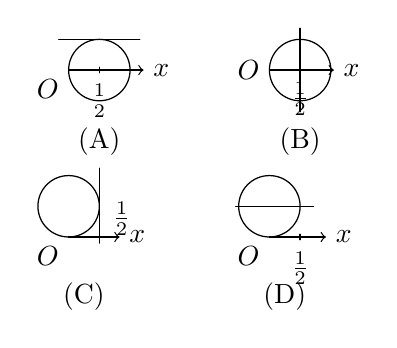
\begin{tikzpicture}[x=0.78cm,y=0.78cm,line width=0.45pt,line cap=round]
  % (A) rho=cos(theta) 对应圆心 (1/2,0)、半径 1/2；上方水平线相切。
  \begin{scope}
    \draw (0.5,0) circle (0.5);
    \draw (-0.16,0.5) -- (1.16,0.5);
    \draw[->] (0,0) -- (1.22,0) node[right] {$x$};
    \node[below left] at (0,0) {$O$};
    \draw (0.5,-0.045) -- (0.5,0.045);
    \node[below] at (0.5,-0.07) {$\frac12$};
    \node[below] at (0.5,-0.78) {(A)};
  \end{scope}

  % (B) 同一圆，x=1/2 直线通过圆心。
  \begin{scope}[xshift=2.55cm]
    \draw (0.5,0) circle (0.5);
    \draw (0.5,-0.68) -- (0.5,0.68);
    \draw[->] (0,0) -- (1.05,0) node[right] {$x$};
    \node[left] at (0,0) {$O$};
    \node[below] at (0.5,-0.04) {$\frac12$};
    \node[below] at (0.5,-0.78) {(B)};
  \end{scope}

  % (C) 干扰图：圆底端为 O，右侧竖线与圆相切。
  \begin{scope}[yshift=-2.12cm]
    \draw (0,0.5) circle (0.5);
    \draw (0.5,-0.10) -- (0.5,1.12);
    \draw[->] (0,0) -- (0.83,0) node[right] {$x$};
    \node[below left] at (0,0) {$O$};
    \node[right] at (0.56,0.30) {$\frac12$};
    \node[below] at (0.25,-0.58) {(C)};
  \end{scope}

  % (D) 干扰图：圆底端为 O，水平线通过圆心。
  \begin{scope}[xshift=2.55cm,yshift=-2.12cm]
    \draw (0,0.5) circle (0.5);
    \draw (-0.55,0.5) -- (0.72,0.5);
    \draw[->] (0,0) -- (0.92,0) node[right] {$x$};
    \node[below left] at (0,0) {$O$};
    \draw (0.5,-0.045) -- (0.5,0.045);
    \node[below] at (0.5,-0.08) {$\frac12$};
    \node[below] at (0.25,-0.58) {(D)};
  \end{scope}
\end{tikzpicture}
\end{center}
\nopagebreak[4]
\end{question}
\begin{question}
\gkti{11}从正方体的 6 个面中选取 3 个面，其中有 2 个面不相邻的选法共有\mbox{（　　）}

(A) 8 种　　(B) 12 种　　(C) 16 种　　(D) 20 种

\end{question}
\begin{question}
\gkti{12}据 2002 年 3 月 5 日九届人大五次会议《政府工作报告》：“2001 年国内生产总值达到 95933 亿元，比上年增长 7.3\%”，如果“十·五”期间（2001 年—2005 年）每年的国内生产总值都按此年增长率增长，那么到“十·五”末我国国内年生产总值约为\mbox{（　　）}

(A) 115000 亿元　　(B) 120000 亿元　　(C) 127000 亿元　　(D) 135000 亿元

\end{question}
\gkpart{二、填空题}

\begin{question}
\gkti{13}椭圆 $5x^2+ky^2=5$ 的一个焦点是 $(0,2)$，那么 $k=\underline{\qquad}$。

\end{question}
\begin{question}
\gkti{14}$(x^2+1)(x-2)^7$ 展开式中 $x^3$ 的系数是$\underline{\qquad}$。

\end{question}
\begin{question}
\gkti{15}已知 $\sin\alpha=\cos2\alpha$，$\alpha\in\left(\dfrac\pi2,\pi\right)$，则 $\tan\alpha=\underline{\qquad}$。

\end{question}
\begin{question}
\gkti{16}已知 $f(x)=\dfrac{x^2}{1+x^2}$，那么
\nopagebreak[4]
\[f(1)+f(2)+f\left(\frac12\right)+f(3)+f\left(\frac13\right)+f(4)+f\left(\frac14\right)=\underline{\qquad}\text{。}\]

\end{question}
\gkpart{三、解答题}

\begin{question}
\gkti{17}已知复数 $z=1+i$，求实数 $a,b$ 使
\nopagebreak[4]
\[az+2b\overline{z}=(a+2z)^2\text{。}\]

\end{question}
\begin{question}
\gkti{18}设 $\{a_n\}$ 为等差数列，$\{b_n\}$ 为等比数列，$a_1=b_1=1$，$a_2+a_4=b_3$，$b_2b_4=a_3$，分别求出 $\{a_n\}$ 及 $\{b_n\}$ 的前 10 项的和 $S_{10}$ 及 $T_{10}$。

\Needspace{0.4\textheight}
\end{question}
\begin{question}
\gkti{19}四棱锥 $P-ABCD$ 的底面是边长为 $a$ 的正方形，$PB\perp$ 平面 $ABCD$。

(1) 若面 $PAD$ 与面 $ABCD$ 所成的二面角为 $60^\circ$，求这个四棱锥的体积；

(2) 证明无论四棱锥的高怎样变化，面 $PAD$ 与面 $PCD$ 所成的二面角恒大于 $90^\circ$。

\textbf{原页图位：}四棱锥示意图标出顶点 $P,A,B,C,D$；底面边 $AB$、$BC$ 为虚线，$PB$ 为虚线，$PA$、$PC$、$PD$、$AD$、$CD$ 为实线。
\nopagebreak[4]
\begin{center}% 第 19 题四棱锥示意图，虚实线按固定来源第 1 页重绘；坐标仅控制图形布局。
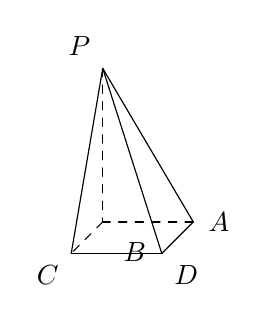
\begin{tikzpicture}[x=1cm,y=1cm,line width=0.42pt,line cap=round,line join=round]
  \coordinate (B) at (0,0);
  \coordinate (A) at (1.15,0);
  \coordinate (C) at (-0.40,-0.40);
  \coordinate (D) at (0.75,-0.40);
  \coordinate (P) at (0,1.95);

  % 虚线：PB、AB、BC。
  \draw[dashed] (P) -- (B);
  \draw[dashed] (A) -- (B);
  \draw[dashed] (B) -- (C);

  % 实线：PA、PC、PD、AD、CD。
  \draw (P) -- (A);
  \draw (P) -- (C);
  \draw (P) -- (D);
  \draw (A) -- (D);
  \draw (C) -- (D);

  \node[above left=1pt] at (P) {$P$};
  \node[right=2pt] at (A) {$A$};
  \node[below right=4pt] at (B) {$B$};
  \node[below left=1pt] at (C) {$C$};
  \node[below right=1pt] at (D) {$D$};
\end{tikzpicture}
\end{center}
\nopagebreak[4]
\end{question}
\begin{question}
\gkti{20}设 $A\text{、}B$ 是双曲线
\nopagebreak[4]
\[
x^2-\frac{y^2}{2}=1
\]
上的两点，点 $N(1,2)$ 是线段 $AB$ 的中点。

(1) 求直线 $AB$ 的方程；

(2) 如果线段 $AB$ 的垂直平分线与双曲线相交于 $C\text{、}D$ 两点，那么 $A\text{、}B\text{、}C\text{、}D$ 四点是否共圆？为什么？

\Needspace{0.4\textheight}
\end{question}
\begin{question}
\gkti{21}(1) 给出两块相同的正三角形纸片（如图 1、图 2），要求用其中一块剪拼成一个三棱锥模型，另一块剪拼成一个正三棱柱模型，使它们的全面积都与原三角形的面积相等。请设计一种剪拼方法，分别用虚线标示在图 1、图 2 中，并作简要说明；

(2) 试比较你剪拼的正三棱锥与正三棱柱的体积的大小；

(3) 如果给出的是一块任意三角形的纸片（如图 3），要求剪拼成一个直三棱柱，使它的全面积与给出的三角形的面积相等。请设计一种剪拼方法，用虚线标示在图 3 中，并作简要说明。

\textbf{原页图位：}图 1、图 2 为两块相同正三角形轮廓，图 3 为任意三角形轮廓；原图没有剪切虚线，供作答者自行标示。
\nopagebreak[4]
\begin{center}% 第 21 题原页图：只重绘三块空白三角形轮廓；原卷没有预印剪线。
\begin{tikzpicture}[x=0.78cm,y=0.78cm,line cap=round,line join=round,
  outline/.style={draw=black,line width=0.55pt}]
  % 图 1、图 2：正三角形轮廓。
  \draw[outline] (1,1.732) -- (0,0) -- (2,0) -- cycle;
  \node[below=2pt] at (1,-0.03) {图 1};

  \begin{scope}[xshift=2.35cm]
    \draw[outline] (1,1.732) -- (0,0) -- (2,0) -- cycle;
    \node[below=2pt] at (1,-0.03) {图 2};
  \end{scope}

  % 图 3：按原页比例重绘任意三角形示意轮廓。
  \begin{scope}[xshift=4.75cm]
    \draw[outline] (0.75,1.75) -- (0,0) -- (4,0) -- cycle;
    \node[below=2pt] at (2,-0.03) {图 3};
  \end{scope}
\end{tikzpicture}
\end{center}
\nopagebreak[4]
\end{question}
\begin{question}
\gkti{22}已知 $a>0$，函数 $f(x)=ax-bx^2$。

(1) 当 $b>0$ 时，若对任意 $x\in\mathbb R$ 都有 $f(x)\leqslant1$，证明：$a\leqslant2\sqrt b$；

(2) 当 $b>1$ 时，证明：对任意 $x\in[0,1]$，$|f(x)|\leqslant1$ 的充要条件是 $b-1\leqslant a\leqslant2\sqrt b$；

(3) 当 $0<b\leqslant1$ 时，讨论：对任意 $x\in[0,1]$，$|f(x)|\leqslant1$ 的充要条件。

\end{question}